\section{Introduction}
\label{sec:intro}

The advent of modern generative diffusion models---spanning Latent Diffusion Models (LDMs)~\cite{ldm}, Diffusion Transformers (DiTs)~\cite{dit}, and Rectified Flow-Matching architectures~\cite{flux}---has democratized photorealistic image synthesis. In particular, generative inpainting has become ubiquitous in consumer editing software, enabling users to seamlessly insert, alter, or erase complex objects from digital photographs via natural language prompts. While these tools facilitate benign digital content creation, they also introduce severe security vulnerabilities, facilitating deceptive media manipulation, forged legal and insurance evidence, and sophisticated misinformation campaigns. Detecting and localizing these local manipulations is therefore a foundational requirement for digital media authentication and image forensics.

Unlike whole-image synthesis, where global structural incoherence, geometric warping, and unnatural perspective cues frequently betray synthetic origin, local generative inpainting modifies only a constrained sub-region of an otherwise authentic photograph. Consequently, over $90\%$ of the image content may remain pristine, preserving natural lens distortion, camera sensor noise, and scene lighting. At the same time, state-of-the-art diffusion inpainters condition their generation on surrounding context, synthesizing textures that harmoniously integrate with adjacent authentic pixels. Forensic detectors must therefore identify subtle sub-pixel boundary seams and micro-statistical noise discrepancies without relying on macroscopic semantic distortions.

Figure~\ref{fig:intro-problem} illustrates the problem using an inpainted image and its reference annotation. The input image provides the scene context, while the colored annotation identifies the localized area the system is expected to find. In practice, the annotation is available for evaluation but is not supplied to the detector when examining an unknown image. This distinction makes both the image-level decision and the accuracy of the predicted region important.

\begin{figure*}[t]
\centering
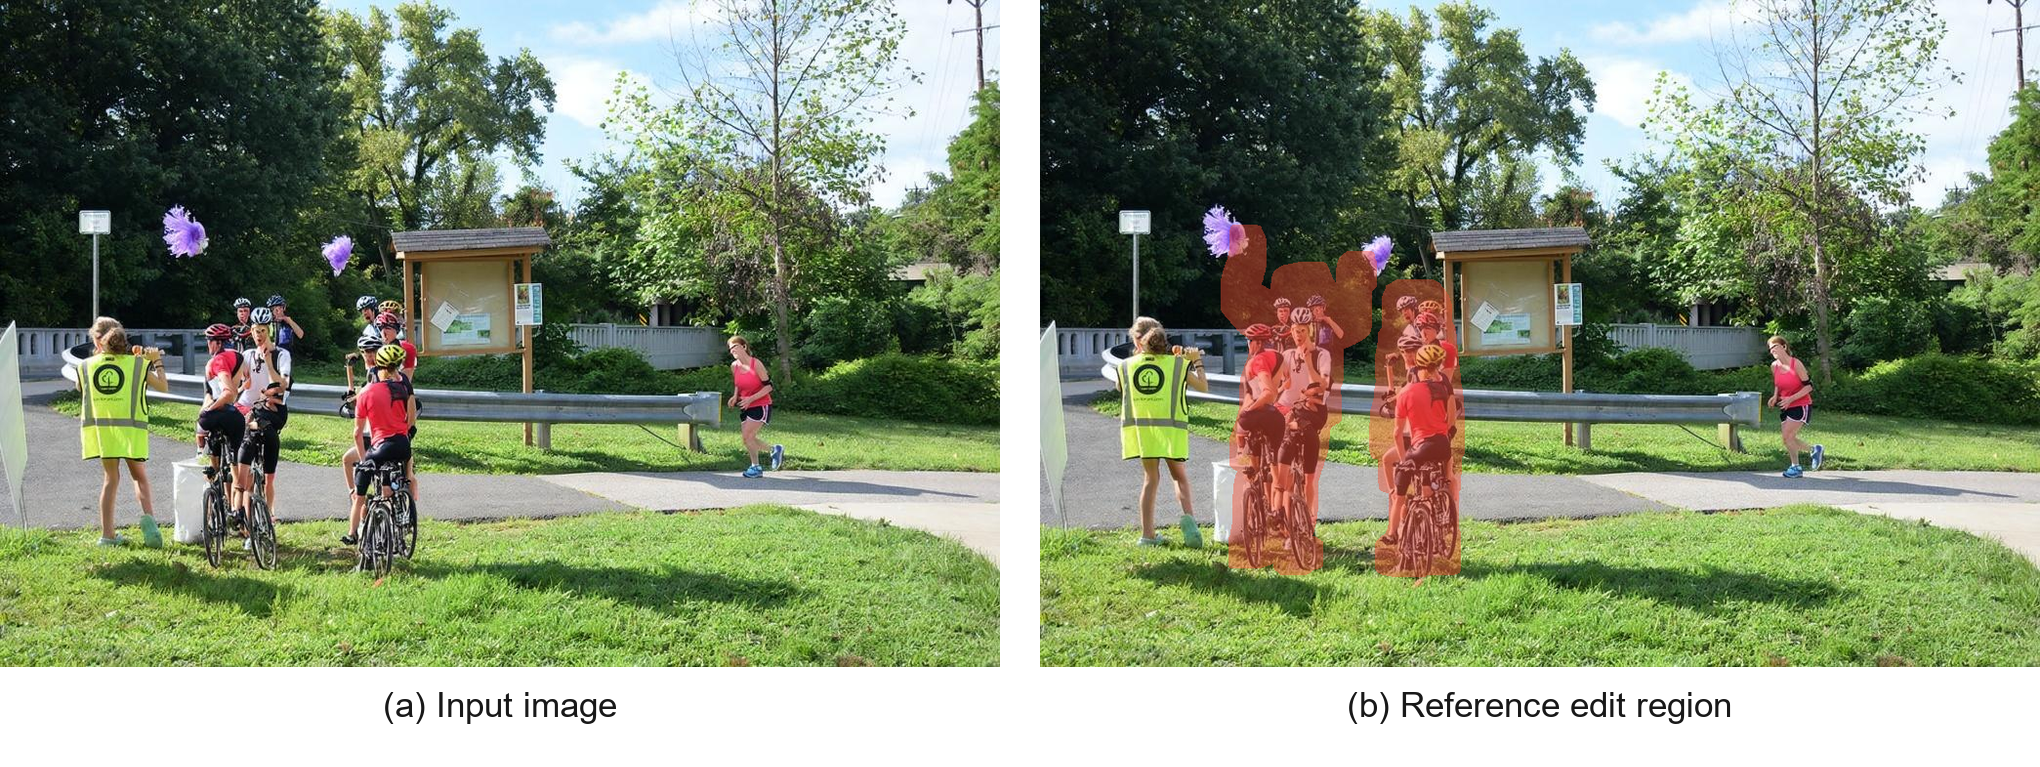
\includegraphics[width=0.92\textwidth]{figures/introduction_problem.png}
\caption{An example of the local inpainting detection and localization problem. (a) An edited input image from the OpenSDID-derived development data. (b) The same image with the reference edit region overlaid in red. The reference mask is shown for illustration and evaluation; it is not an input to the detector.}
\Description{An image of cyclists is shown alongside the same image with its annotated edited region highlighted in red.}
\label{fig:intro-problem}
\end{figure*}

Under these operational constraints, prior research in image edit detection has predominantly pursued two disjoint and inherently flawed paradigms:
\begin{enumerate}
    \item \textbf{Global Downsampling Paradigms:} The first paradigm resizes the entire input image to a fixed low-resolution canvas (e.g., $224 \times 224$ or $512 \times 512$) to fit within standard convolutional or Vision Transformer (ViT) backbones~\cite{opensdi,fused,cnndet}. While this provides complete macroscopic scene context, bilinear or bicubic downsampling acts as a spatial low-pass filter, catastrophically smoothing away the high-frequency pixel interpolation seams and diffusion noise variances that characterize generative inpainting boundaries. As a result, downsampling-based models fail on modern high-resolution generators such as SDXL and FLUX.1, where inpainting artifacts are inherently high-frequency and localized.
    \item \textbf{Patch-Centric Paradigms without Global Context:} The second paradigm processes native-resolution local crops to preserve microscopic details~\cite{trufor,mvss}. However, evaluating crops in isolation strips the model of global semantic context. High-frequency pristine textures---such as dense foliage, fine fabric weaves, asphalt, or halftone printing screens---exhibit localized residual energy comparable to synthetic boundaries, causing unconstrained crop detectors to suffer from catastrophic false-positive rates on authentic imagery. Furthermore, historical crop-training regimes assigned global whole-image labels to random crops, poisoning classifiers by penalizing models when background crops from edited images contained zero manipulated pixels.
\end{enumerate}

To overcome this fundamental scale-context dichotomy, this paper presents \textbf{FRAME} (\textbf{F}orensic \textbf{R}esidual \textbf{A}ttention with \textbf{M}ulti-scale \textbf{E}vidence), an end-to-end framework for joint single-image inpainting detection and pixel-level localization. FRAME unifies global macroscopic context and microscopic local fidelity through a dual-view hierarchy. At inference, a single suspect image is parsed into both a resized whole-image view ($512 \times 512$) and an overlapping grid of native-resolution sliding tiles ($512 \times 512$ with stride 256) at 1:1 pixel scale. Each view is processed by a Tri-Stream encoder combining dense hierarchical representations from ConvNeXt-Base, self-supervised foundation tokens from frozen DINOv2-Base, and a 60-channel noise residual pyramid combining fixed Spatial Rich Model (SRM) filters and learned Bayar constrained convolutions.

To fuse these complementary modalities, we formulate a Multi-Head Cross-Attention Decoder (MH-CAD) wherein high-pass forensic residual tokens act as queries to cross-attend to dense semantic keys and values. This dynamic interaction ensures that high-frequency noise anomalies are promoted only when they coincide with non-semantic boundary disruptions, effectively suppressing false alarms on natural textures. Finally, we formulate a joint dual-view training objective with balanced Dice and Binary Cross-Entropy (BCE) loss alongside clean-image suppression penalties, resolving historical supervision noise and widening the decision boundary separation between authentic and manipulated images by $4.3\times$.

The primary contributions of this work are summarized as follows:
\begin{enumerate}
    \item \textbf{Dual-View Native-Resolution Architecture:} We design a unified detection and localization pipeline that couples a resized global view for macroscopic scene reasoning with an overlapping $1:1$ native-resolution sliding tile grid, eliminating the spatial information loss caused by fixed-canvas downsampling while preserving sub-pixel boundary detail.
    \item \textbf{Tri-Stream Forensic Feature Extraction:} We formulate a complementary three-stream encoder combining hierarchical spatial representations from ConvNeXt-Base, self-supervised semantic tokens from frozen DINOv2-Base, and a 60-channel noise residual pyramid (30 fixed SRM + 30 learnable Bayar filters) to capture structural semantics and micro-texture noise anomalies simultaneously.
    \item \textbf{Multi-Head Cross-Attention Decoder (MH-CAD):} We develop a top-down feature pyramid decoder where forensic queries attend to dense semantic context across multiple scales, coupled with Stride-2 high-pass refinement, preventing false alarms on high-frequency pristine textures while sharpening tiny inpainting masks.
    \item \textbf{Joint Dual-View Supervision \& State-of-the-Art Benchmark:} We establish a balanced multi-task training objective that decouples whole-image classification from crop-level presence, eliminating the historical 100\% false-alarm vulnerability. On the multi-generator OpenSDID benchmark across five diffusion families (SD 1.5, 2.1, 3, SDXL, and FLUX.1), FRAME achieves \textbf{91.20\% image accuracy}, \textbf{92.60\% balanced accuracy}, \textbf{93.40\% AUROC}, and \textbf{47.30\% mean localization IoU}, surpassing FUSED, MaskCLIP, and DeCLIP across all metrics.
\end{enumerate}
